\section{Modeling}
\label{sec:modeling}


% %
% SYSTEM DESCRIPTION
% %
We consider the environment sketched in Figure~\ref{fig:modeling-system-sketch}, which is characterized by:

\begin{itemize}
	\item  \textbf{workload:} mobile devices send to the system tasks that can be partitioned in two classes $C_{1}$ and $C_{2}$.
	\item \textbf{system:} a two-tiers system, made of:	
	\begin{itemize}
		\item a remote Cloud server with virtually unlimited servants.
		\item a Cloudlet with $N$ servants, having the ability to off-load tasks to the Cloud, accordingly to a certain \textit{off-loading policy} parametrized by a given \textit{threshold}.
	\end{itemize}
\end{itemize}

\begin{figure}
	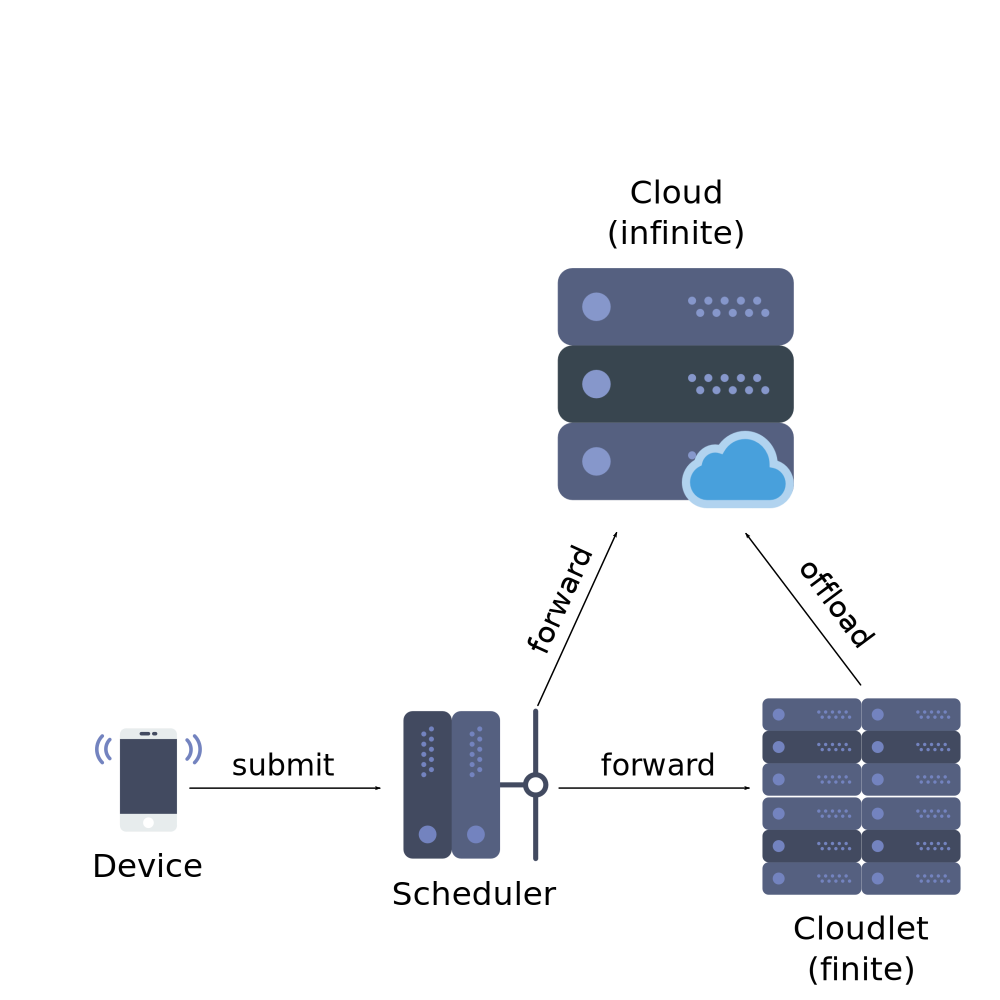
\includegraphics[width=\columnwidth]{fig/modeling-system-sketch}
	\caption{The system sketch.}
	\label{fig:modeling-system-sketch}
\end{figure}

We assume that
(i) the Cloudlet provides tasks with higher service rate than the Cloud, 
(ii) when a task is interrupted in the Cloudlet and it is sent to the Cloud, the restart process comes with a \textit{setup time overhead}.

% %
% GOALS AND OBJECTIVES
% %
\paragraph{Goals and Objectives}
The main goals of the simulation are about system tuning.
In particular, we propose to determine with a $95\%$ level of confidence
\begin{itemize}
	\item the response time as a function of the threshold $S$,
	\item the throughput as a function of the threshold $S$,
	\item the distribution of the response time when $S=N$ and
	\item the threshold of the off-loading policy that minimizes the response time.
\end{itemize}


% %
% CONCEPTUAL MODEL
% %
\paragraph{Conceptual Model}
The conceptual model is depicted in Figure~\ref{fig:modeling-conceptual-model}.

\begin{figure}
	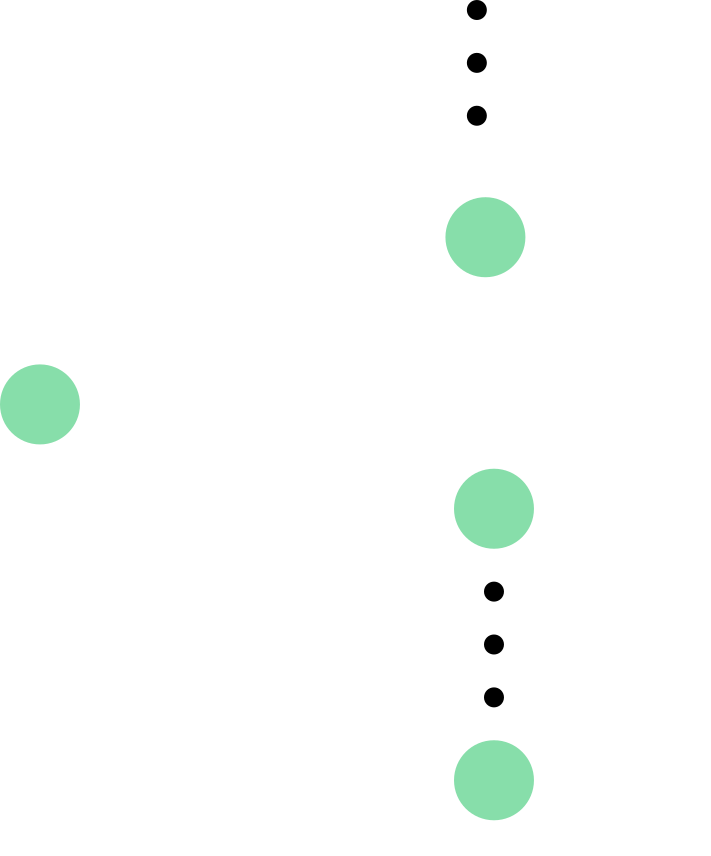
\includegraphics[width=\columnwidth]{fig/modeling-conceptual-model}
	\caption{The conceptual model.}
	\label{fig:modeling-conceptual-model}
\end{figure}

% %
% SPECIFICATION MODEL
% %
\paragraph{Specification Model}
The state of a system is a comprehensive characterization of the system at a particular time.
The state of the system is represented by the pair $(n_{clt,1},n_{clt,2},n_{cld,1},n_{cld,2})$, where $n_{cld,i}$ is the number of tasks belonging to the $i$-th class within the Cloudlet and $n_{cld,i}$ is the number of tasks belonging to the $i$-th class within the Cloud.
An event is an occurrence that could change the state of the system at the event time, according to the event type.
Our events are ...

Tasks belonging to the first class, i.e. $t\in C_{1}$ arrive to the system with an exponential arrival process with rate $ \lambda_{1}$; whilst tasks belonging to the seconds class, i.e. $t\in C_{2}$ arrive to the system with an exponential arrival process with rate $ \lambda_{2}$.
The Cloudlet serves tasks belonging to the first class with exponentially distributed service time with rate $\mu_{cld,1}$; whilst the Cloudlet serves tasks belonging to the second class with exponentially distributed service time with rate $\mu_{cld,2}$.
The Cloud serves tasks belonging to the first class with exponentially distributed service time with rate $\mu_{clt,1}$; whilst the Cloudlet serves tasks belonging to the second class with exponentially distributed service time with rate $\mu_{clt,2}$.
We assume that 
(i) $\mu_{clt,i}>\mu_{cld,i}\ \forall i=1,2$ and
(ii) the setup time $T_{setup}$ is exponentially distributed with expected value $E[T_{setup}]$.

\begin{algorithm}
	\SetAlgoLined
	\If{task of class 1}{
		\If{$n_{clt}=N$}{
			send on the Cloud
		} 
		\If{$n_{clt}+n_{cld}<S$}{
			accept
		} 
		\eIf{$n_{cld} > 0$}{
			accept the task on the Cloudlet and send a class 2 task on the Cloud
		}{
		accept the task on the Cloudlet
		}
	}
	\If{arrival of class 2}{
		\eIf{$n_{clt}+n_{cld}>=S$}{
			send on the Cloud
		}{
		accept the task on the Cloudlet
	}
	}
	\caption{The dispatching policy.}
	\label{alg:modeling-dispatching-policy}
\end{algorithm}

% %
% COMPUTATIONAL MODEL
% %
\paragraph{Computational Model}
The proposed performance model has been implemented as a Python application. 
The simulation parameters can be configured with a simple YAML file that can be loaded by the simulation program.
The full open source code is available at \cite{gmarciani-pydes} and some representative configurations and outputs are presented in Section~\ref{sec:usage}.

We adopted the next-event simulation paradigm, using 
(i) a custom multi-stream Lehmer generator to generate random events, whose parameters have been described in Section~\ref{sec:random-number-generation} and whose evaluation will be presented in Section~\ref{sec:evaluation}; and
(ii) a priority-queue based calendar with the ability both to schedule and un-schedule events.

Even if both the initial and terminal state can have any possible value, we adopted the convention of initializing and terminating the system in the idle state $(0,0,0,0)$. In particular, the terminal state is reached via the well-known closed door technique driven by a stop time condition.

The calendar is initialized by scheduling the first arrival in the initialization phase. The submission of an arrival $a$ to the system could induce
(i) the scheduling of the corresponding completion event,
(ii) the scheduling of a new arrival, or
(iii) the unscheduling of a previously scheduled completion, i.e. interruption in Cloudlet.

The next-event calendar is implemented as priority queue, appropriately extended to manage scheduling/unscheduling of events and exclusion of impossible events, i.e. arrivals with occurrence time greater than the stop time.
The impossibility of events is managed by letting the calendar contain possible events only, which is the best approach when the event list is assumed to be very long.


% %
% VERIFICATION
% %
\paragraph{Verification}
The model has been verified by 
\begin{itemize}
	\item \textbf{flow consistency:} responsible to verify the correctness of flow trends, such as:
	
	\begin{equation}
	n_{cld,i}=a_{cld,i}-c_{cld,i}-s_{cld,i}
	\end{equation}
	\begin{equation}
	n_{cld,i}=a_{cld,i}-c_{cld,i}+s_{cld,i}
	\end{equation}
	\begin{equation}
	s_{clt,i}=s_{cld,i}
	\end{equation}
	
	 where 
	 $n_{j,i}$ is the population of tasks belonging to $i$-th class in the $j$-th subsystem, 
	 $a{j,i}$ is the number of tasks belonging to $i$-th class arrived to the $j$-th subsystem, 
	 $c{j,i}$ is the number of tasks belonging to $i$-th class completed in the $j$-th subsystem, 
	 $s{j,i}$ is the number of tasks belonging to $i$-th class switched from/to the $j$-th subsystem.
	 
	\item \textbf{workload change consistency:} responsible to verify the correctness of metrics variations in response to arrival/service rates variations, such as:
	
	\begin{equation}
		\lambda_{1}' > \lambda_{1} \Rightarrow
	\end{equation}
	
	\item \textbf{stationary check:} responsible to verify the correctness of the model in stationary conditions.
\end{itemize}

% %
% VALIDATION
% %
\paragraph{Validation}
It is well-known that model development should includes a final validation step. Clearly, we cannot conduct this final step because we cannot compare the performance model with its real counterpart.